\chapter{Compactness}
\section{Sequentially Compact}
\dfn{Sequentially Compact}{Let $(X,d)$ be a metric space. $X$ is called sequentially compact if every sequence in $X$ has a convergent subsequence. (Often applied to a subset $S$ of $X$)}
\nt{For $S$ to be sequentially compact the limit of subsequence must be in $S$}
\dfn{Boundedness}{A subset $S$ of $(X, d)$ is bounded if $S \subset B_r(x)$ for some $x \in X$ and $r > 0$}
\nt{Boundedness depends on the metric but if two metrics are ``equivalent" analogous to norms)}
\begin{Theorem}{}{}
	A subset $K$ of $\bbR^n$ is sequentially compact $\iff$ $K$ is closed and bounded
\end{Theorem}
\begin{myproof}
	Proof in steps
	\begin{enumerate}
		\item \label{hnbsc: step 1}\subsubsection{A closed interval $\bs{[a, b]}$ in
			      $\bbR$ is sequentially compact}\parinn
		      \begin{myproof}
			      Given a sequence $x_1 , x_2 , \cdots$  in $\bbR$ in $[a, b]$ we can extract a monotonic subsequence as follows:

			      We call $x_i$ to be a peak if $x_i > x_j$ $\forall\ j > i$. Now there are two cases. If number of peaks is infinite then the next peak comes after the previous one so smaller than the previous one. So its a strictly decreasing sequence. If number of peaks are finite then at some point we cant find a peak with this property that means no matter which term i peak there is at least one term after that which is greater than or equal to that term. $y_1 = $a term after the last peak. and $y_{i+1} = $a term after $y_i$ such that $y_{i+1} \geq y_i$. Hence $y_1 , y_2 ,\cdots$ is a weakly increasing	sequence.

			      When $\{x_n\}$ contained in $[a, b]$ by boundedness of the monotonic subsequence, it converges to its sup/inf and the limit is in $[a, b]$
		      \end{myproof}
		\item \label{hnbsc: step 2}\subsubsection{$\bs{[a_1,b_1]\times [a_2,b_2]\times \cdots \times [a_n,b_n]\subset \bbR^n}$ is sequentially compact (w.r.t $\bs{p-}$norm for $\bs{p=1,2,\infty}$. Later for any norm)}

		      \begin{myproof}

			      Recall a sequence $\{x_m\}\to x$ in $\bbR^n$ $\iff$ The sequence converges in each coordinate i.e. $x_{m_i}\to x_i$

			      Take a sequence in the given box. Extract a subsequence whose entries in 1st slot converge (necessarily to $x_i$ in $[a_1,b_1]$ by \hyperref[hnbsc: step 1]{step 1} From this sequence, extract a further subsequence whose entries	in
			      second slot converge to $x_2\in [a_2,b_2]$. Continue \end{myproof}

		\item \label{hnbsc: step 3}\subsubsection{Every closed subset of a sequentially compact set is sequentially compact}\parinn
		      \begin{myproof}
			      Exercise
		      \end{myproof}

		      This will show each closed and bounded subset of the Euclidean Space $\bbR^n$ is sequentially compact. (because such a set will be contained in a box)
		\item \label{hnbsc: step 4}\subsubsection{If K is sequentially compact then K is closed and bounded}\parinn
		      \begin{myproof}
			      If $K$ is not closed then some limit point $x$ of $K$ will not be in $K$. Then there is a sequence $\{y_m\}$ in $K$ converges to $x\notin K$  violating sequential compactness of $K$.

			      If $K$ is not bounded take $\{x_m\}\in K$ with $\|x_m\|\geq n$ then $\{x_m\}$ can not be convergent
		      \end{myproof}
	\end{enumerate}
\end{myproof}
\nt{\hyperref[hnbsc: step 4]{Step 4} works for any metric space. Then we need to have a ball instead of norm}
\begin{Theorem}{}{}
	If $K$ is a sequentially compact of a metric space $X$, then $K$ is closed and bounded
\end{Theorem}
\begin{myproof}
	Same argument as \hyperref[hnbsc: step 4]{step 4} use $x_m$ such that $d(x_m,x)\geq m$
\end{myproof}
\qs{}{If $K$ is closed and bounded in $(X, d)\implies K$ is sequentially compact}
\sol{No. Any counter-example. Define a metric on real number which induces same topology as the	normal topology in such a way that there is a closed and bounded set that is not compact.}
\qs{}{
	\begin{enumerate}
		\item If $V$, $W$ are normed linear spaces can we define a norm on $V\times W$ ?
		\item If $V$, $W$ are metric spaces can we define a metric on $V\times W$ ?
		\item If $V$, $W$ are topological spaces can we define a topology on $V\times W$ ?
	\end{enumerate}
}
\section{Open Cover and Compactness}
\dfn{Open Cover}{
Let $\{V_{\alpha}\}_{\alpha\in I}$  be a family of subsets of metric space $X$ we say that $\{V_{\alpha}\}_{\alpha\in I}$ is a cover of $X$ if $\bigcup\limits_{\alpha} V_{\alpha}=X$ and we say that $\{V_{\alpha}\}_{\alpha\in I}$  is an open cover if each $V_{\alpha}$ is open (in $X$)
}
\dfn{Compact}{
$X$ is called compact if each open cover of $X$ has a finite subcover i.e.	$\{V_{\alpha_1},V_{\alpha_2},\cdots , V_{\alpha_n}\}\subset	\{V_{\alpha}\}_{\alpha\in I}$ with $V_{\alpha_1}\cup V_{\alpha_2}\cup \cdots	\cup V_{\alpha_n}=X$
}

\nt{\begin{enumerate}
		\item \parinn This definition makes sense for any topological space $X$.

		      If $X$ is a metric space then it is a fact that $X$ is compact $\iff$ $X$ is		sequentially compact. This is not true for general topological spaces. Both		implications fail.
		\item \parinn Reformulation of compactness for subset $K$ of $X$ in terms of		open sets of $X$
		      \begin{center}
			      \begin{tabular}{p{2.1cm}p{1cm}p{11cm}}
				      $K$ is compact & $\iff$ & Every cover of $K$ bt open sets of $K$ has a	finite subcover.                                                                                                                                                                                                               \\
				      \multicolumn{3}{c}{As open sets of $K$ are precisely (open sets of $X)\cap	K$. We have the following}                                                                                                                                                                                                 \\
				      $K$ is compact & $\iff$ & For any family $\{V_{\alpha}\cap K\}_{\alpha\in I}$ where $V_{\alpha}$ are open in $X$ whose union is $K$, there is a finite	subcover.                                                                                                                                      \\
				                     & $\iff$ & For any family $\{V_{\alpha}\cap K\}_{\alpha\in I}$ of open sets	in $X$ such that $\bigcup\limits_{\alpha\in I}V_{\alpha} \supset K$, there must	be a finite subfamily $V_{\alpha_1},V_{\alpha_2},\cdots,V_{\alpha_n}$ with			$\bigcup\limits_{i=1}^nV_{\alpha_i}\supset K$
			      \end{tabular}
		      \end{center}
		      If i take this definition of compactness of a subset $K$ of metric space $X$	then $K$ is compact as subset of $X$ $\iff$ $K$ is compact as a subset of it	itself
	\end{enumerate}}
\begin{Theorem}{Haine Borel Theorem}{hnb}
	\begin{center}
		\begin{tabular}{rcl}
			$K\subset \bbR^n$ is compact & $\iff$ & $K$ is closed and boundeded
		\end{tabular}
	\end{center}
	(w.r.t $p=1,2$ or $\infty$ norm as they are equivalent.)
\end{Theorem}
\begin{myproof}
	\subsubsection{Only If Part:-}
	Proof in steps
	\begin{enumerate}[label=\bfseries\tiny\protect\circled{\small\arabic*}]
		\item \label{hnb:st1}Closed interval $[a,b]$ is compact in $\bbR$. \textbf{\textit{Proof:}} \hyperref[th:hnb:s1]{Theorem \ref{th:hnb:s1}}
		\item \label{hnb:st2}Closed box $[a_1,b_1]\times [a_2,b_2]\times\cdots\times
			      [a_n,b_n]$ is compact in $\bbR^n$. \textbf{\textit{Proof:}} \hyperref[th:hnb:s2]{Theorem \ref{th:hnb:s2}}
		\item \label{hnb:st3}A closed subset of a compact set is compact. \textbf{\textit{Proof:}} \hyperref[th:hnb:s3]{Theorem \ref{th:hnb:s3}}
	\end{enumerate}
	These steps would give the backward direction of \hyperref[th:hnb]{Haine Borel	Theorem} i.e. suppose $K$ is closed and bounded in $\bbR^n$ $\implies$ $K\in [-M.M]^n\implies $ compact by \ref{hnb:st2}

	\subsubsection{If Part:-}
	\textbf{Bounded:} First we have to show that $K$ is compact $\implies K$ is	bounded an i.e. $K\subset B_r(x)$ in $(X,d)$ for some $x\in X$, $r>0$

	Consider open cover $\{B_n(x)\}_{n\in\bbZ^+}$ of $X$ and hence of $K$. This must 	have a finite subcover $B_{n_1}(x),B_{n_2}(x)_,$ $\cdots ,B_{n_k}(x)$. Take $r=\max\{n_1,n_2,\cdots,n_k\}$ Hence $$K\text{ is compact }\implies K\text{ is
			closed}$$

	\parinf\textbf{Closed: }\parinn We will show that $X\setminus K$ is open. Pick $x\notin K$. Enough to construct an open neighborhood $U_x\ni x$ such that $U_x\cap x=\phi$

	Take $z\in K$. Let $c=d(x,z)$ then \begin{center}
		\begin{tabular}{cccl}
			$B_{\frac{c}{3}}(x)$ & $\cap$ & $B_{\frac{c}{3}}(z)=\phi$ & by triangle
			inequality                                                              \\
			$\parallel$          &        & $\parallel$               &             \\
			$W_z$                &        & $V_z$                     &
		\end{tabular}
	\end{center}
	\begin{center}
		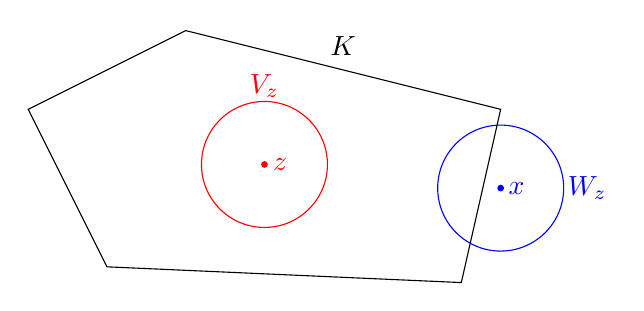
\begin{tikzpicture}
			\draw (-1,0) -- (-2,2) -- (0,3) -- (4,2) node[xshift=-2cm,yshift=8mm]{$K$} --
			(3.5,-0.2) --cycle;
			\draw[red] (1,1.3) node[yshift=1cm]{$V_z$} circle (0.8cm);
			\draw[red, fill=red] (1,1.3) node[xshift=2mm]{$z$} circle (1pt);
			\draw[blue] (4,1)node[xshift=1.1cm]{$W_z$} circle (0.8cm);
			\draw[blue, fill=blue] (4,1) node[xshift=2mm]{$x$} circle (1pt);
		\end{tikzpicture}
	\end{center}
	Now $\bigcup\limits_{z\in K}V_z\supset K$. So $\{V_z\}$ is an open cover of $K$.
	By compactness we have $V_{z_1}\cup V_{z_2}\cup \cdots\cup V_{z_n}\supset K$.

	\begin{center}
		\begin{tikzpicture}
			\draw[red] (1,0)node[xshift=-1.3cm]{$V_{z_1}$} circle (1cm);
			\draw[red] (4,0)node[xshift=1.4cm,yshift=-5mm]{$W_{z_1}$} circle (1cm);
			\draw[blue] (1.5,1)node[xshift=-9mm,yshift=1cm]{$W_{z_2}$} circle (1cm);
			\draw[blue] (3.5,-1)node[xshift=1.3cm,yshift=-5mm]{$V_{z_1}$} circle (1cm);
			\draw[myg] (3.7,1)node[xshift=1.6cm,yshift=1.1cm]{$V_{z_3}$} circle (1.6cm);
			\draw[myg] (1.5,-2)node[xshift=-2cm]{$W_{z_3}$} circle (1.6cm);

		\end{tikzpicture}
	\end{center}
	As $W_z\cap V_z=\phi$ $\forall z\in K$.  We have $\underbrace{\left( W_{z_1}\cup
			W_{z_2}\cup \cdots \cup W_{z_n}\right) }_{\substack{\text{Finite intersection
				of}\\ \text{open neighborhoods of } x,\\ \text{so call this }U_x}}\cap K=\phi$
\end{myproof}

Key fact that made this work: For $x\neq z$ in $X$, we could find open neighborhoods of $V$ and $W$ (of $x$ and $z$ respectively) such that $V\cap W=\phi$. Topological spaces that satisfy this property are called \label{housdorff}Housdorff.

What we proved is the following
\begin{Theorem}{}{}
	For a Housdorff Topological space $X$ any compact subset $K$ is closed and bounded
\end{Theorem}

\begin{Theorem}{}{hnb:s3}
	$C$ is a closed subset of compact set $X$ $\implies $ $C$ is compact.
\end{Theorem}
\begin{myproof}
	Take any open cover $\{V_{\alpha}\}_{\alpha\in I}$ of $C$by open sets in $X$ i.e $\bigcup\limits_{\alpha}V_{\alpha}\supset C$. Now $\opensets \cup \{X\setminus C\}$ is an open cover of $x$. We have a finite subcover by compactness of $X$. The same subcover (after dropping $X\setminus C$ if necessary) works for $C$.
\end{myproof}
\wc{Closed interval $\bs{[a,b]}$ is compact in $\bs{\bbR}$}{Suppose $\opensets$ is an open cover of $[a,b]$ by open sets in $\bbR$.

Hence every one of the points in the interval is covered by one of the $V_{\alpha}$. Hence there is some interval contained in the $V_{\alpha}$
\begin{center}
	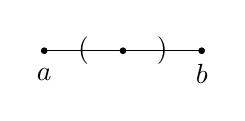
\begin{tikzpicture}
		\draw (-1,0) -- (1,0);
		\draw[fill=black] (-1,0) node[yshift=-3mm]{$a$} circle (1pt);
		\draw[fill=black] (1,0) node[yshift=-3mm]{$b$} circle (1pt);
		\draw (-0.5,0) node{$($};
		\draw (0.5,0) node{$)$};
		\draw[fill=black] (0,0) circle (1pt);
	\end{tikzpicture}
\end{center}
So i could just ignore the $V_{\alpha}$  and say for each point in the interval we can get an open interval that is part of a $V_{\alpha}$. So how can i find a subcover. I could simply travel from one end to the other.

So i start with $a$ so $a$ must be contained in some open interval
\begin{center}
	\begin{tikzpicture}
		\draw (-1,0) -- (1,0);
		\draw[red,fill=red] (-1,0) node[yshift=-3mm]{$a$} circle (1pt);
		\draw[fill=black] (1,0) node[yshift=-3mm]{$b$} circle (1pt);
		\draw[red] (-1.4,0) node{$($};
		\draw[red] (-0.6,0) node{$)$};
		\draw[<-,red] (-0.6,-0.2) -- (-0.6,-0.5) node[xshift=1mm,yshift=-2mm]{$\delta_1$};
	\end{tikzpicture}
\end{center}
Not only that i have covered up a small segment of the closed interval, upto a point, $a+\delta_1$. Say $[a,a+\delta_1)\subset V_1$.

Let $a+\delta_1$ is contained in some open interval which is contained in $V_2$ upto the point $a+\delta_2$
\begin{center}
	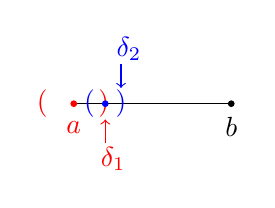
\begin{tikzpicture}
		\draw (-1,0) -- (1,0);
		\draw[red,,fill=red] (-1,0) node[yshift=-3mm]{$a$} circle (1pt);
		\draw[fill=black] (1,0) node[yshift=-3mm]{$b$} circle (1pt);
		\draw[red] (-1.4,0) node{$($};
		\draw[red] (-0.6,0) node[xshift=-0.2mm]{$)$};
		\draw[<-,red] (-0.6,-0.2) -- (-0.6,-0.5) node[xshift=1mm,yshift=-2mm]{$\delta_1$};
		\draw[blue] (-0.8,0) node{$($};
		\draw[blue] (-0.4,0) node{$)$};
		\draw[<-,blue] (-0.4,0.2) -- (-0.4,0.5) node[xshift=1mm,yshift=2mm]{$\delta_2$};
		\draw[blue,fill=blue] (-0.6,0) circle (1pt);
	\end{tikzpicture}
\end{center}
Now continue.
\tcbline\parinf
What is wrong with this ?\parinn

We could have smaller and smaller intervals. For example length of first interval can be $\frac13$, length of second interval can be $\frac19$, length of third interval can be $\frac1{27}$ and so on. So its a geometric progression and it will sum less than 1. So i just may not get there in finite number of steps.

}

\qs{}{Suppose $X$ is a topological space that is compact and \ref{housdorff} (Take $x$ ro be a compact metric space if you like). Prove that given disjoint compact subsets $K$ and $L$, there are disjoint open sets $U$ and $V$ with $K\subset U$ and $L\subset V$(First do it for $K=$ single point)}
In the above exercise we could have replaced the word compact with another word which is closed because $X$ is given to be compact so any closed set will be compact and in a Housdorff space compact subset is also closed.
\nt{Cauchy Sequence in Metric space need not converge. For example $(0,1)$ and take the sequence $\frac1n$. It wants to converge to 0 but 0 is not there.}


\begin{Theorem}{\hyperref[th:hnb]{Haine Borel Theorem} - If Part: \hyperref[hnb:st1]{Step \ref{hnb:st1}}}{hnb:s1}
	$[0,1]$ is compact in $\bbR$
\end{Theorem}
\begin{myproof}
	Let $\opensets$ be a family of open sets in $\bbR$ covering $[0,1]$.

	Let $S=\{a\in [0,1]\mid [0,a]\text{ can be covered by a finite number of }V_{\alpha}\text{'s}\}$. Our goal is to prove $1\in S$.

	Let $0\leq x<y\leq 1$. So $[0,x]\subset [0,y]$. This $y\in S\implies x\in S$ i.e $x\notin S\implies y\notin S$. Now $S$ is nonempty because $0\in S$ and $S$ is bounded. Let $u=\lub$ of $S$. Clearly $0\leq u\leq 1$. Hence it is enough to show $u=1$ and $u\in S$.

	$0\in$ some open set $V_{\alpha}$. Hence $\exists\ \eps>0$ $B_{\eps}(0)\subset \oset$. Hence $\forall$ point $x\in [0,\eps)$ $x\in S$

	For $a\in[0,u)$, $a\in S$ (otherwise $a$ itself would be an upper bound for $S$). As $\opensets$ cover $[0,1]$, $u\in V_{\beta}$. So $\exists \ \eps>0$ such that $(u-\eps,u+\eps)\subset V_{\beta}$ As $u-\eps\in S$ we have $\opset{1}\sup\opset{2}\sup\cdots\opset{k}\supset [0,u-\eps]$ Then $\opset{\beta}\cup\opset{1}\cup\opset{2}\cup \cdots\opset{k}\supset \left[0,u+\frac{\eps}{2}\right]$. So $u=1$ because otherwise some $u+\delta\in S$ contradicting that $u$ is an upper bound.
\end{myproof}
\qs{}{Can the strategy from the last time be made to work ti actually extract a finite subcover of a given cover.}
\begin{Theorem}{}{}
	Suppose $X\xrightarrow{f} Y$ continuous and $K\subset X$ is compact. Then $f(K)$ is compact
\end{Theorem}
\begin{myproof}
	Let $\opensets$ be an open cover of $f(k)$ by open sets $V_{\alpha}$ of $Y$. So $$\bigcup\limits_{\alpha}V_{\alpha} \supset f(K)\implies f^{-1}\left(\bigcup\limits_{\alpha}V_{\alpha}\right)=\bigcup\limits_{\alpha}f^{-1}\left(V_{\alpha}\right)\supset f^{-1}(f(K))\supset K$$ Thus $\left\{f^{-1}(V_{\alpha})\right\}_{\alpha\in I}$ is an open (because of continuity \hyperref[th:cont:invofopen]{Theorem \ref{th:cont:invofopen}}) cover of $K$.

	Extract a finite subcover \begin{align*}
		         & f^{-1}\left(V_{\alpha_1}\right)\cup f^{-1}\left(V_{\alpha_2}\right) \cup \cdots f^{-1}\left(V_{\alpha_m}\right)\supset K \\
		\implies & f\left(f^{-1}\left(V_{\alpha_2}\right) \cup \cdots f^{-1}\left(V_{\alpha_m}\right)\right)\supset f(K)                    \\
		\implies & \bigcup_{i=1}^m f\left(f^{-1}\left(V_{\alpha_i}\right)\right)\supset f(K)
	\end{align*}
	As $V_{\alpha_i}\supset f\left(f^{-1}\left(V_{\alpha_i}\right)\right)$ we have $\bigcup\limits_{i=1}^mV_{\alpha_i}\supset f(K)$
\end{myproof}
\qs{}{$f(\text{Sequentially compact }K)\text{ is sequentially compact}$}


\begin{Theorem}{\hyperref[th:hnb]{Haine Borel Theorem} - If Part: \hyperref[hnb:st2]{Step \ref{hnb:st2}}}{hnb:s2}
	$K=[a_1,b_1]\times[a_2,b_2]\times \cdots\times [a_n,b_n]$ is compact in $\bbR^n$
\end{Theorem}
\begin{myproof}
	Induction on $n$. $n=1$ we already proved in \hyperref[th:hnb:s1]{Theorem \ref{th:hnb:s1}}.Let $\mcF=\opensets$ be a cover of $K$ by open sets in $\bbR^n$. Fix $u\in [a_1,b_1]$ and consider  $\{u\}\times \underbrace{[a_2,b_2]\times \cdots\times [a_n,b_n]}_{\substack{=C\text{ is compact}\\\text{by induction on }n}}$ Hence $\{u\}\times C$ is compact because   $\bbR^{n-1}\to\bbR^n$ which maps $(y_2,y\cdots,y_n)\mapsto (u,y_2,\cdots,y_n)$ or $ {f(C)=\{u\}\times C} $ is continuous.

	For each $p=(u,y_2,\cdots,y_n)$ in $\{u\}\times C$ pick an open neighborhood $V_p\in \mcF$. Hence $V_{p}\supset (x-\eps,x+\eps)\times \underbrace{(y_2-\eps,y_2+\eps)\times \cdots\times (y_n-\eps,y_n+\eps)}_{W_p}$ for some $\eps=\eps_p$ depending on $p$
	\begin{center}
		\begin{tikzpicture}
			\draw (0.5,5)node[yshift=-5.3cm]{$a_1$} rectangle (6,0)node[yshift=-0.3cm]{$b_1$};
			\draw (3,0) node[yshift=-0.3cm]{$u$} -- (3,5);
			\draw[blue] (2.5,0) rectangle (3.5,5);
			\draw[red] (1.5,0) rectangle (4.5,3);
			\draw[red,fill=red] (3,1.5) circle (1pt);
			\draw[red] (2.3,2.5) rectangle (3.7,3.9);
			\draw[red,fill=red] (3,3.2) circle (1pt);
			\draw[red]  (2.2,5) rectangle (3.8,3.4);
			\draw[red,fill=red] (3,4.2) circle (1pt);
		\end{tikzpicture}
	\end{center}
	By compactness of $\{u\}\times C$, extract a finite subcover of the cover $\{W_p\}$. Hence $W_{p_1}\cup W_{p_2}\cup\times \cup W_{p_k}\supset \{u\}\times C$. Since its a union of open sets we have in fact $W_{p_1}\cup W_{p_2}\cup\times \cup W_{p_k}\supset (u-\eps,u+\eps)\times C$ where $\eps=\min\{\eps_{p_1},\eps_{p_2},\cdots,\eps_{p_k}\}$. Let $\mcF_u=\{V_{p_1},V_{p_2}<\cdots,V_{p_k}\}$. So $$V_{p_1}\cup V_{p_2}\cup \cdots\cup V_{p_k}\supset W_{p_1}\cup W_{p_2}\cup\cdots\cup W_{p_k}\supset (u-\eps,u+\eps)\times C$$i.e. this finite subcover $\mcF_u$ cover not just the slice but a tube around it.

	Now as $u$ varies in $[a_1,b_1]$, $(u-\eps_u,u+\eps_u)$ gives an open cover. Extract a finite subcover  $(u_1-\eps_{u_1},u_1+\eps_{u_1}),(u_2-\eps_{u_2},u_2+\eps_{u_2}),\cdots,(u_l+\eps_{u_l},u_l+\eps_{u_l})$ . Then $\mcF_{u_1}\cup\mcF_{u+2}\cup\cdots\cup\mcF_{u_l}$ is a finite subcover of $[a_1,b_1]\times C=K$
\end{myproof}
\qs{}{Why the map $\bbR^{n-1}\to\bbR^n$ which maps $(y_2,y\cdots,y_n)\mapsto (u,y_2,\cdots,y_n)$ or $ {f(C)=\{u\}\times C} $ is continuous ?}
\qs{}{$X,Y$ are topological spaces. $K\subset X$ and $Y\subset Y$ are compact subsets. Then $K\times L$ is compact subset of $X\times Y$ where Open sets of $X\times Y$ are $\bigcup$(Open set of $X$)$\times$(Open set in $Y$)}

\begin{Theorem}{}{all norms equiv}
	All norms on $\bbR^n$ are equivalent
\end{Theorem}
\begin{myproof}
	Enough to show any norm $f \sim \norm$  \begin{align*}
		 & \text{i.e }\alpha \|u\|\leq f(u)\leq \beta\|u\| \forall\ u                        \\
		 & \text{i.e } \alpha \leq \frac{f(u)}{\|u\|}\leq \beta\ \forall\ u \forall\ u\neq 0
	\end{align*}
	Note that $\frac{f(x)}{\|x\|}=f\left(\frac{x}{\|x\|}\right)=f(u)$ where $u=\frac{x}{\|x\|}$, so $\|u\|=1$. Hence it is enough to show that $$\alpha\leq f(u)\leq \beta$$for any $u$ with $\|u\|=1$

	Let $S=\{u\mid \|u\|=1\}$ is the unit sphere in $\bbR^n$, which is closed and bounded

	\begin{center}
		\begin{tabular}{rcl}
			$S$ is closed and bounded & $\implies$ & $S$ is compact                                        \\
			                          & $\implies$ & $f(S)$ is compact in $\bbR$                           \\
			                          & $\implies$ & $f(S)$ is closed and bounded in $\bbR$                \\
			                          & $\implies$ & $f(S)$ has largest element in $\beta$ and smallest    \\
			                          &            & element $\alpha$ such that $\alpha\leq f(S)\leq\beta$
		\end{tabular}
	\end{center}
\end{myproof}


